%Measurements that affect the decisions made by a node in the network. TCP itself relies on active measurements, such as tracking RTT:s of segments.

\section{Improving TCP Startup Performance with Active Measurements}

We will now demonstrate how active measurements can be used to improve the TCP start up algorithm. We will closely follow the the work of Ningning Hu and P. Steenkiste~\cite{Hu03} in introducing the \textit{paced start} algorithm, a proposed replacement for the \textit{slow start} algorithm.

In TCP slow start, the congestion window size is exponentially increased until a packet is lost or the congestion window size reaches a predefined value of \textit{ssthresh}, in order to find out a suitable congestion window size. This often results in considerable number of lost packets. The packet stream emitted by the algorithm is also quite bursty, which may cause load spikes in the router queues of the network. The load spikes increase packet losses of other connections in the network~\cite{Hu03}.    

In paced start algorithm, the PTR (Packet Transmission Rate) method~\cite{Hu03b} is used to estimate the available bandwidth of the path. In the PTR method, the source machine sends a sequence of packet trains, starting with a tiny inter-packet-gap in the initial packet train. The average inter-packet-gap of the ACK-packet-trains from the target machine will be measured. The source machine will repeatedly adjust its inter-packet-gap based on the measured inter-packet-gap of the target machine, and keep sending new packet trains, until its inter-packet-gap equals the measured inter-packet-gap of the target machine. At this point, the source machine and the target machine are processing packages at approximately the same rate. This rate will be the estimate for the available bandwidth on the path. Figure~\ref{fig:PTR}, by Ningning Hu and P. Steenkiste~\cite{Hu03}, illustrates the workings of the PTR method.

\begin{figure}
	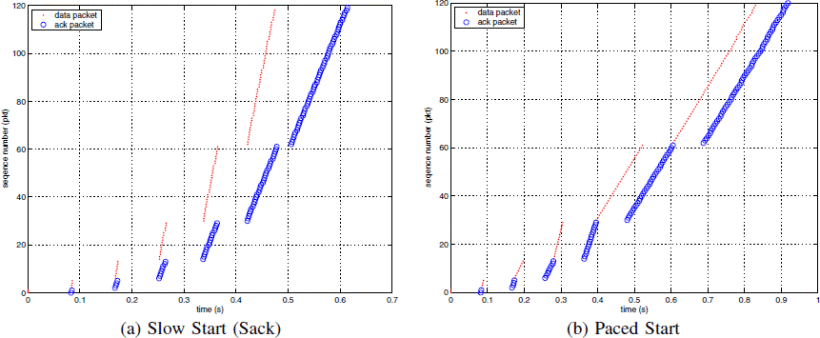
\includegraphics[width=0.5\textwidth]{images/hu03_PTR.png}
	\caption{Figure taken from~\cite{Hu03}. Packet trains of source and target machines plotted against time for both slow start and paced start algorithm. The data is from a simulation with roundtrip time of 80ms, a bottleneck link of 5Mb/s and available bandwidth of 3Mb/s. In plot (b), the difference of the inter-packet-gaps of the packet trains from source and the target machines converges, yielding the estimate for the available bandwidth. This convergence is visualised in the slopes of the blue and red lines becoming equal.}
	\label{fig:PTR}
\end{figure}

The paced start algorithm has two major differences to the slow start. First, the paced start algorithm is not self clocking (arrival of an ACK triggers the sending of a package), because in a self clocking setup the sent and received packets are not evenly paced. Instead, the paced start only sends a new packet train after the previous packet train has been entirely acknowledged. Secondly, 

%the difference between the spacing in the data packets and the acknowledgement packets is used to infer information about the bandwidth of the route.


%Alternatively this subsection could be a separate section.